\documentclass{beamer}

\usepackage[utf8]{inputenc}
\usepackage[T1]{fontenc}

\usepackage[english]{babel}
\usepackage{amsmath}
\usepackage{cleveref}
\usepackage{amssymb}
\usepackage{mathtools}

%%Numbers, expectation
\newcommand{\N}{\mathbb{N}}
\newcommand{\E}{\mathbb{E}}
\renewcommand{\P}{\mathbb{P}}
\newcommand{\Var}{\mathbb{V}}
\newcommand{\R}{\mathbb{R}}
\newcommand{\D}{\mathcal{D}}
\newcommand{\B}{\mathcal{B}}
\newcommand{\Dh}{\D_h}
\renewcommand{\phi}{\varphi}
\newcommand*\diff{\mathop{}\!\mathrm{d}} % integral

%% mathoperator
\DeclareMathOperator*{\argmax}{arg\,max}
\DeclareMathOperator*{\argmin}{arg\,min}
\DeclareMathOperator*{\dom}{dom}
\DeclareMathOperator*{\sign}{sign}
\DeclareMathOperator*{\diag}{diag}

\DeclareMathOperator*{\Cov}{Cov}
\DeclareMathOperator*{\Cor}{Corr}
\DeclareMathOperator*{\Id}{Id}

%proximal operator
\newcommand{\prox}[3][]{\operatorname{prox}^{#1}_{#2}\left(#3 \right)}

\usepackage{xcolor}

%% sort citations by increasing number
\usepackage[sort,nocompress]{cite}

\usepackage{graphicx}% http://ctan.org/pkg/graphicx
\graphicspath{{../figures/}{../../figures}{../../memes}} %Setting the graphicspath
\usepackage{caption,subcaption}

\usepackage{tikz}
\usepackage{pgfplots}
\usetikzlibrary{backgrounds}
\usetikzlibrary{intersections}
\usepgfplotslibrary{fillbetween}

% \usepackage[right]{showlabels}


%%
\theoremstyle{plain}
\newtheorem{prop}{Proposition}[section]
\newtheorem{algo}{Algorithm}[section]
\newtheorem{assumption}{Assumption}
\theoremstyle{remark}
\newtheorem{remark}{Remark}[section]

% cref
\crefname{assumption}{Assumption}{Assumptions}
\crefname{equation}{}{}

\usepackage{autonum}

\usepackage{bm} %% bold math symbols

\usepackage{bbm} %% for \mathbbm{1}


% algorithmic environment
\usepackage{algorithm}
\usepackage[noend]{algpseudocode}

% for some reason this was required on one void linux installation (but not the other)
\usepackage{sansmathaccent}
\pdfmapfile{+sansmathaccent.map}

\author{Axel Böhm}

% shows which section we're in
\usetheme{Darmstadt}

% page number
\setbeamertemplate{footline}[frame number]
\setbeamercolor{page number in head/foot}{fg=gray}


% display things like onslide or visible already before but grayed out
\setbeamercovered{transparent}

% set the itemize item symbol as a diamond
\setbeamertemplate{itemize item}{$\diamond$}
% set the itemize subitem symbol as a triangle
\setbeamertemplate{itemize subitem}{$\blacktriangleright$}

% set the enumerate item symbol as a roman numbers
\setbeamertemplate{enumerate item}{(\roman{enumi})}


\author{Axel Böhm}

% shows which section we're in
\usetheme{Darmstadt}

% page number
\setbeamertemplate{footline}[frame number]
\setbeamercolor{page number in head/foot}{fg=gray}


% display things like onslide or visible already before but grayed out
\setbeamercovered{transparent}

% set the itemize item symbol as a diamond
\setbeamertemplate{itemize item}{$\diamond$}
% set the itemize subitem symbol as a triangle
\setbeamertemplate{itemize subitem}{$\blacktriangleright$}

% set the enumerate item symbol as a roman numbers
\setbeamertemplate{enumerate item}{(\roman{enumi})}


\title{Projected Gradient Descent}

\begin{document}
\maketitle
\frame{\tableofcontents}

\section{Introduction}%



\begin{frame}
  \frametitle{Constrained Optimization}

  \begin{minipage}{0.5\textwidth}
    \begin{block}{Constrained optimization problem}
      \begin{equation}
        \begin{aligned}
          \text{minimize } & f(x)\\
          \text{subject to } & x\in C
        \end{aligned}
      \end{equation}
      \textcolor{blue}{How to solve them}
      \begin{itemize}
        \item Project onto $C$
        \item transform to \textit{unconstrained problem}
      \end{itemize}
    \end{block}
  \end{minipage}
  \begin{minipage}{0.45\textwidth}
    \begin{figure}[ht]
      \centering
      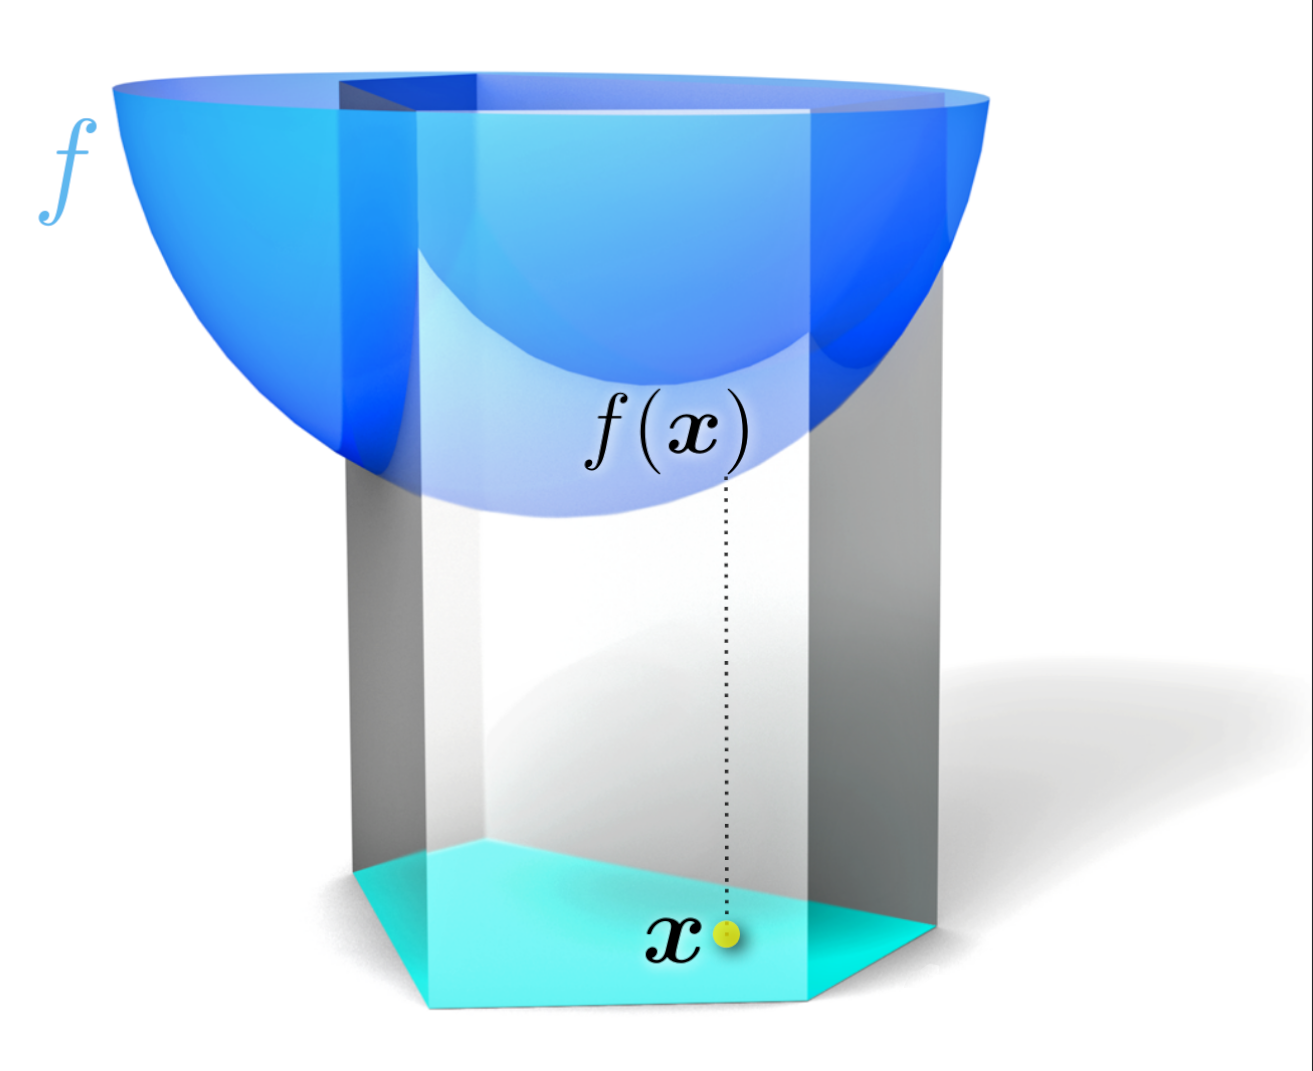
\includegraphics[width=\textwidth,height=\textheight,keepaspectratio]{constrained_3d}
      % \caption{\label{fig:label} }
    \end{figure}
  \end{minipage}
\end{frame}


\begin{frame}
  \frametitle{Constrained Optimization}

  \begin{minipage}{0.5\textwidth}
    \begin{block}{Constrained optimization problem}
      \begin{equation}
        \begin{aligned}
          \text{minimize } & f(x)\\
          \text{subject to } & x\in C
        \end{aligned}
      \end{equation}
      \end{block}
      \textcolor{blue}{We will focus on:}
      \begin{itemize}
        \item \textbf{Projected Gradient Descent}
      \end{itemize}
  \end{minipage}
  \begin{minipage}{0.45\textwidth}
    \begin{figure}[ht]
      \centering
      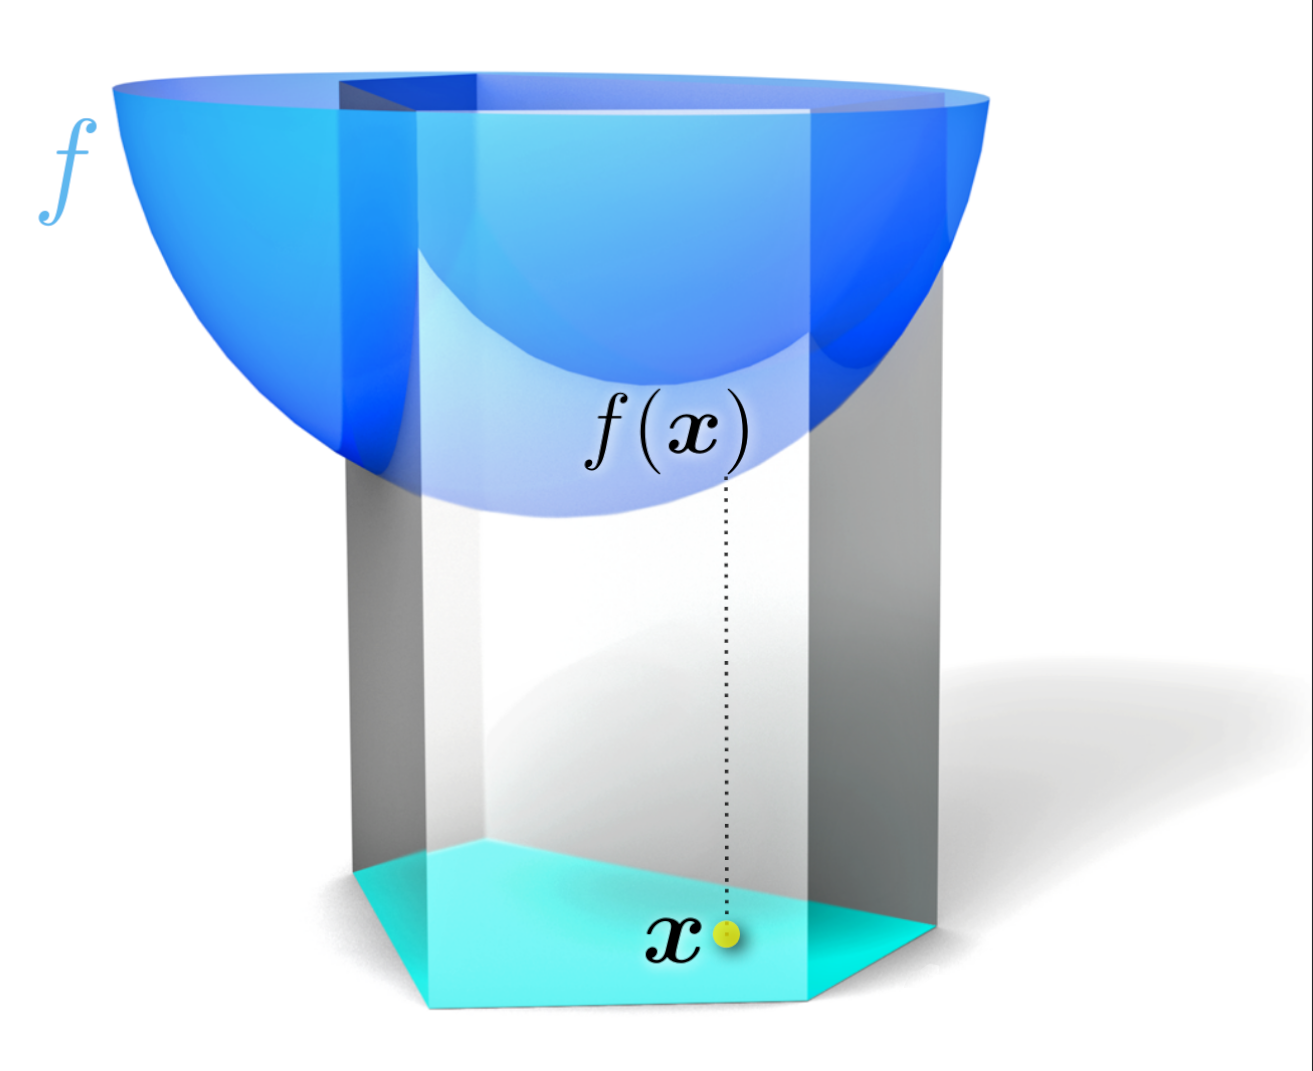
\includegraphics[width=\textwidth,height=\textheight,keepaspectratio]{constrained_3d}
      % \caption{\label{fig:label} }
    \end{figure}
  \end{minipage}
\end{frame}

\section{Projection}%
\label{sec:}

\begin{frame}
  \frametitle{Projected Gradient Descent}

  \textcolor{blue}{Idea:} After every step project back onto the set: $\Pi_C(x) :=\argmin_{y\in C} \Vert y-x \Vert$.

    \begin{figure}[ht]
      \centering
      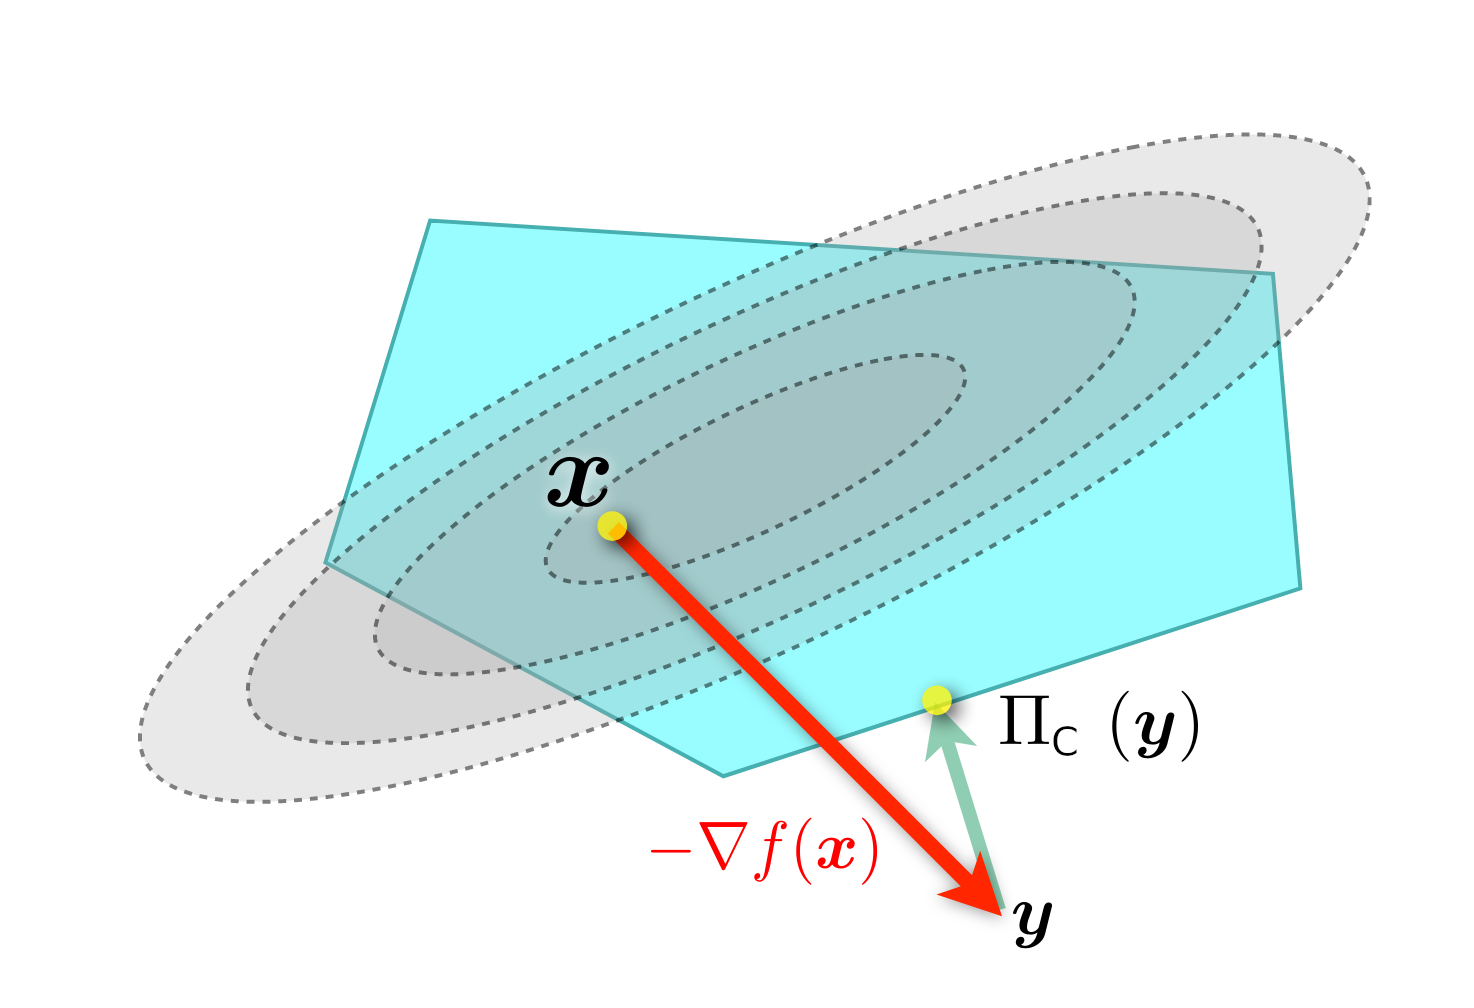
\includegraphics[width=\textwidth,height=0.7\textheight,keepaspectratio]{test}
      % \caption{\label{fig:label} }
    \end{figure}

\end{frame}


\begin{frame}
  \frametitle{Projected subgradient method}
  \begin{equation}
    \text{(constrained setting)} \quad \min_{x\in C}\, f(x)
  \end{equation}
  \begin{algorithm}[H]
    \caption{Projected subgradient method}\label{label:}
    \begin{algorithmic}[1]
      \For{$k=0, 1, \dots$}
      \State{Pick $g_k \in \partial f(x_k)$}
      \State{$y_{k+1} =  x_k- \alpha g_k $}
      \State{$x_{k+1} = \Pi_C(y_{k+1})$}
      \EndFor
    \end{algorithmic}
  \end{algorithm}
\end{frame}


\begin{frame}
  \frametitle{Properties of the Projection}
  \begin{block}{Fact}
    Let $C\subseteq \R^d$ be closed and convex, $x\in C$ and $y \in \R^d$.Then
    \begin{itemize}
      \item $\langle x- \Pi_C(y), y - \Pi_C(y)  \rangle \le 0$
      \item $\Vert x - \Pi_C(y) \Vert^2 + \Vert y - \Pi_c(y) \Vert^2 \le \Vert y-x \Vert^2$
    \end{itemize}
  \end{block}
  \begin{figure}[ht]
    \centering
    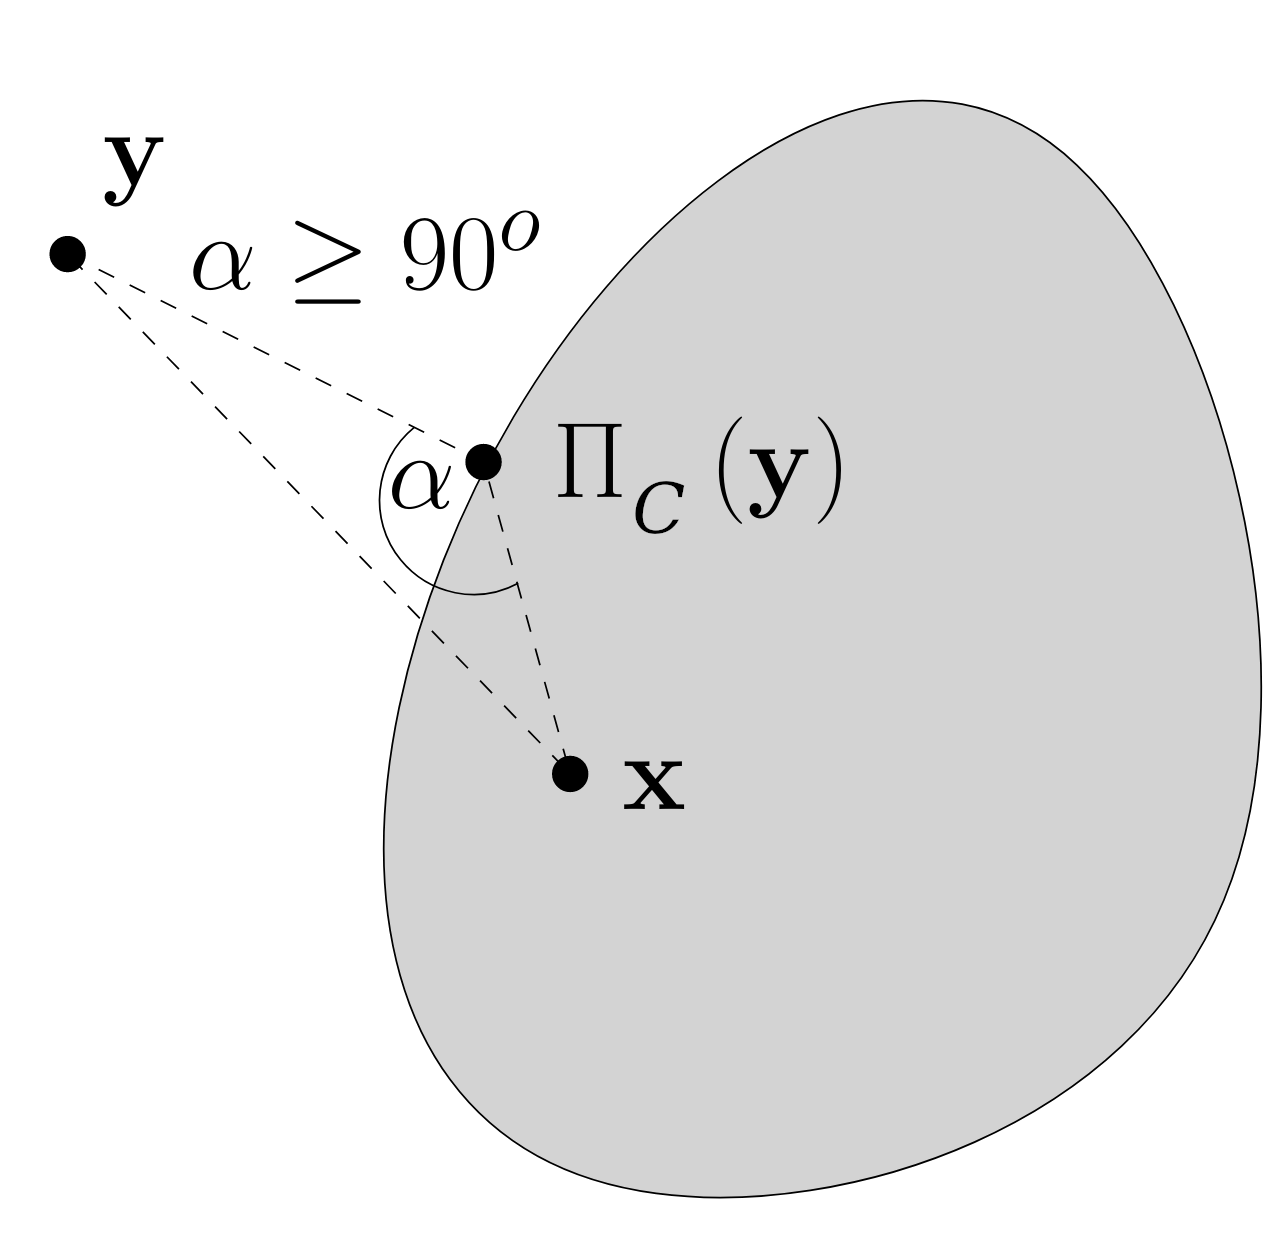
\includegraphics[height=0.5\textheight,keepaspectratio]{projection_property}
    % \caption{\label{fig:label} }
  \end{figure}

\end{frame}


\begin{frame}
  \frametitle{Properties of the Projection}
  \begin{block}{Fact}
    Let $C\subseteq \R^d$ be closed and convex, $x\in C$ and $y \in \R^d$.Then
    \begin{itemize}
      \item $\langle x- \Pi_C(y), y - \Pi_C(y)  \rangle \le 0$
      \item $\Vert x - \Pi_C(y) \Vert^2 + \Vert y - \Pi_c(y) \Vert^2 \le \Vert y-x \Vert^2$
    \end{itemize}
  \end{block}
  \begin{proof}
    Since $\Pi_C(x)$ is the minimizer of a differentiable convex function $d_x(y) =\frac12 \Vert y-x \Vert^2$ over $C$, by the \textbf{first-order optimality condition}
    \begin{align}
      0 &\le \langle \nabla d_x(\Pi_C(x)), y - \Pi_C(x) \rangle \\
        &= \langle \Pi_C(x) - x, y - \Pi_C(x) \rangle
    \end{align}
  \end{proof}
\end{frame}



\begin{frame}
  \frametitle{Results for projected GD}
  For \textbf{closed}, \textbf{convex} set $C\subset \R^d$ \textcolor{blue}{same} number of gradient steps.
  \begin{itemize}
    \item Lipschitz convex function over $C$: $\mathcal{O}(\epsilon^{-2})$ steps
    \item Smooth convex function over $C$: $\mathcal{O}(\epsilon^{-1})$ steps
    \item Smooth and strongly convex over $C$: $\mathcal{O}(\log(\epsilon^{-1}))$
  \end{itemize}

  But:
  \begin{itemize}
    \item Each step requires a projection onto $C$
    \item May or may not be easy to compute
  \end{itemize}

\end{frame}


\begin{frame}
  \frametitle{The projection step: $\Pi_C(x) := \argmin_{y\in C} \Vert y-x \Vert$}
  Computing $\Pi_C(x)$ is an optimization problem itself.

  Efficient in relevant cases:
  \begin{itemize}
    \item Box constraints: $C= [a_1, b_1] \times \dots \times [a_d, b_d]$
    \item Affine subspace (requires solution of system of linear equations)
          \begin{figure}[ht]
            \centering
            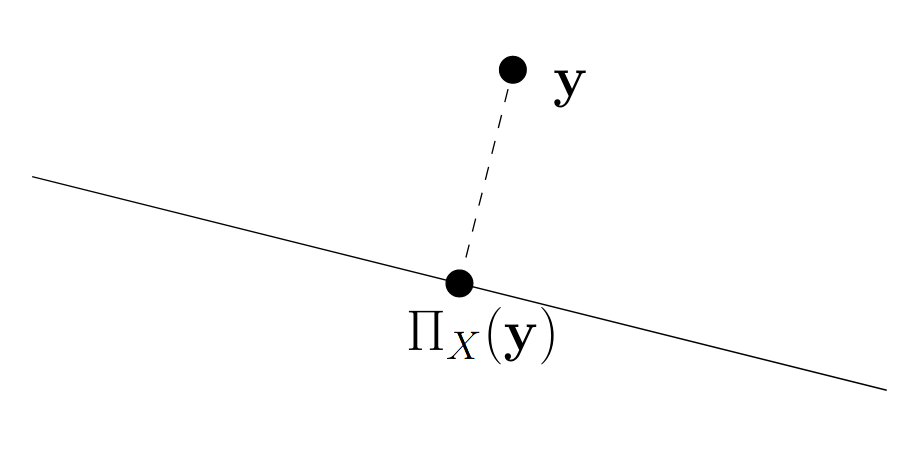
\includegraphics[scale=.12]{projection_onto_affine_space}
          \end{figure}
    \item Projection onto ball with center $c$
          \begin{figure}[ht]
            \centering
            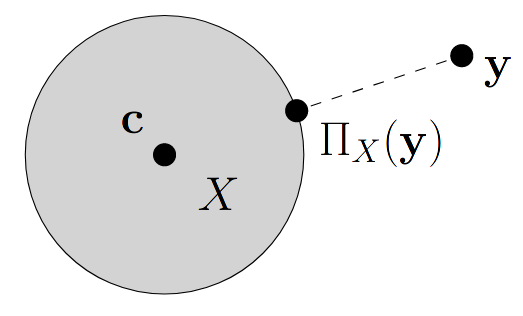
\includegraphics[scale=.2]{projection_onto_ball}
          \end{figure}
  \end{itemize}
\end{frame}


\begin{frame}
  \frametitle{Convergence analysis}
  \begin{proof}
    We can deduce the exact same inequality as before
    \begin{equation}
      \begin{aligned}
        \Vert x_{k+1} - x^* \Vert^2 &= \Vert \Pi_C(x_k - \alpha g_k) - \Pi_C(x^*) \Vert^2 \\
        &\le \Vert x_k - \alpha g_k - x^* \Vert^2 \\
        &= \Vert x_k-x^* \Vert^2 + 2 \alpha \langle g_k, x^*-x_k \rangle + \alpha^2 \Vert g_k \Vert^2\\
        &\le \Vert x_k-x^* \Vert^2 + 2 \alpha (f^* - f(x_k))+ \alpha^2 \Vert g_k \Vert^2.
      \end{aligned}
    \end{equation}
    Continue the proof as in the unconstrained setting.
  \end{proof}
\end{frame}


\section{Proximal Gradient}%
\label{sec:}


\begin{frame}
  \frametitle{Composite minimization problem}

  Consider objective function composed as
  \begin{equation}
    f(x) = g(x) + h(x)
  \end{equation}
  where
  \begin{itemize}
    \item $g$ is \textcolor{blue}{nice}
    \item $h$ is \textcolor{blue}{simple}
  \end{itemize}
  typically we mean nice means smooth. Relevant if $h$ is not differentiable.
  Most notably: Lasso

\end{frame}


\begin{frame}
  \frametitle{Idea}
  Classical gradient step for $g$:
  \begin{equation}
    x_{k+1} = \argmin_{x} g(x_k) + \langle \nabla g(x_k), x-x_k \rangle + \frac{1}{2 \alpha} \Vert x-x_k \Vert^2
  \end{equation}
  Now, for $f= g+h$ we keep this for $g$ and add $h$ \textcolor{blue}{unmodified}:
  \begin{align}
    x_{k+1} &= \argmin_{x} g(x_k) + \langle \nabla g(x_k), x-x_k \rangle + \frac{1}{2 \alpha} \Vert x-x_k \Vert^2 \textcolor{red}{+ h(x)} \\
    &= \argmin_x \frac{1}{2 \alpha} \Vert x - (x_k - \alpha \nabla g(x_k)) \Vert^2 + h(x)
  \end{align}
\end{frame}


\begin{frame}
  \frametitle{The proximal gradient algorithm}

  An iteration is defined as
  \begin{block}{}
  \begin{equation}
    x_{k+1} = \prox{\alpha h}{x_k - \alpha \nabla g(x_k)}
  \end{equation}
  \end{block}
  where the \textcolor{blue}{proximal mapping} for a function $h$ and parameter $\alpha$ is defined as
  \begin{equation}
    \prox{\alpha h}{x} = \argmin_{y \in \R^d} \left\{ h(y) + \frac{1}{2 \alpha} \Vert y-x \Vert^2\right\}.
  \end{equation}


\end{frame}


\begin{frame}
  \frametitle{A generalization of (projected) GD}

  \begin{itemize}
    \item $h \equiv 0$ recovers \textcolor{blue}{gradient descent}.
    \item $h = \chi_C$ recovers \textcolor{blue}{projected gradient descent}
          We call $\chi_C$ the \textbf{indicator function} of $C$
          \begin{align}
            \chi_C&: \R^d \to \R \cup +\infty \\
              & x \mapsto \begin{cases}
                0 & \text{if $x \in C$} \\
                +\infty & \text{otherwise.}
              \end{cases}
          \end{align}
          Proximal mapping becomes
          \begin{equation}
            \prox{\alpha h}{x} = \argmin_{y \in \R^d} \left\{ \chi_C(y) + \frac{1}{2 \alpha} \Vert y-x \Vert^2\right\} = \argmin_{y \in C} \{ \Vert y-x \Vert^2\}.
          \end{equation}
  \end{itemize}
\end{frame}

\begin{frame}
  \frametitle{Convergence}

  Same complexity as GD or projected GD,

  \textcolor{blue}{if we can compute the proximal mapping!}

\end{frame}

\end{document}
